% ***************************************************
% A Classic Thesis Style
% An Homage to The Elements of Typographic Style
%
% Copyright (C) 2012 Andr\'e Miede http://www.miede.de
%
% If you like the style then I would appreciate a postcard. My
% address can be found in the file ClassicThesis.pdf. A collection
% of the postcards I received so far is available online at 
% http://postcards.miede.de
%
% License:
% This program is free software; you can redistribute it and/or
% modify it under the terms of the GNU General Public License as
% published by the Free Software Foundation; either version 2 of
% the License, or (at your option) any later version.
%
% This program is distributed in the hope that it will be useful,
% but WITHOUT ANY WARRANTY; without even the implied warranty of
% MERCHANTABILITY or FITNESS FOR A PARTICULAR PURPOSE.  See the
% GNU General Public License for more details.
%
% You should have received a copy of the GNU General Public
% License along with this program; see the file COPYING.  If not,
% write to the Free Software Foundation, Inc., 59 Temple Place -
% Suite 330, Boston, MA 02111-1307, USA.
%
% ***************************************************************
% Note:
%    * You must not use "u etc. in strings/commands that will be
%      spaced out (use \"u or real umlauts instead)
%    * New enumeration (small caps): \begin{aenumerate}
%      \end{aenumerate}
% 	 * For margin notes: \marginpar or \graffito{}
%    * Do not use bold fonts in this style, it is designed around
%      them
%    * Use tables as in the examples
%    * See classicthesis-preamble.sty for useful commands
% ****************************************************************

\documentclass[ twoside, 
			openright,
			% letterpaper a4paper
			titlepage, 
			numbers=noenddot,
			headinclude, %1headlines
            footinclude=true, 
			cleardoublepage=empty,
			abstractoff, % <--- obsolete, remove (todo)
			BCOR=5mm,
			paper=a4, 
			fontsize=11pt, %11pt,
			]{scrreprt}

%*****************************************************************
% Note: Make all your adjustments in here
%*****************************************************************

\usepackage[backref, backend=biber]{biblatex}
\bibliography{Bibliography}	

% ****************************************************************
% classicthesis-config.tex 
% formerly known as loadpackages.sty, classicthesis-ldpkg.sty, and
% classicthesis-preamble.sty Use it at the beginning of your
% ClassicThesis.tex, or as a LaTeX Preamble in your
% ClassicThesis.{tex,lyx} with % ****************************************************************
% classicthesis-config.tex 
% formerly known as loadpackages.sty, classicthesis-ldpkg.sty, and
% classicthesis-preamble.sty Use it at the beginning of your
% ClassicThesis.tex, or as a LaTeX Preamble in your
% ClassicThesis.{tex,lyx} with % ****************************************************************
% classicthesis-config.tex 
% formerly known as loadpackages.sty, classicthesis-ldpkg.sty, and
% classicthesis-preamble.sty Use it at the beginning of your
% ClassicThesis.tex, or as a LaTeX Preamble in your
% ClassicThesis.{tex,lyx} with \input{classicthesis-config}
% ****************************************************************
% If you like the classicthesis, then I would appreciate a
% postcard. My address can be found in the file
% ClassicThesis.pdf. A collection of the postcards I received so
% far is available online at http://postcards.miede.de
% ****************************************************************

% ****************************************************************
% 1. Configure classicthesis for your needs here, e.g., remove
% "drafting" below in order to deactivate the time-stamp on the
% pages
% ****************************************************************
\PassOptionsToPackage{eulerchapternumbers,
					listings,
					drafting,
				 	pdfspacing,
					floatperchapter,
					%linedheaders,
				 	subfig,
					beramono,
					eulermath,
					parts}{classicthesis}										

% ****************************************************************
% Triggers for this config
% **************************************************************** 
\usepackage{ifthen}
\newboolean{enable-backrefs} % enable backrefs in the bibliography
\setboolean{enable-backrefs}{false} % true false
% TODO backref is incompatible?
% ****************************************************************


% ****************************************************************
% 2. Personal data and user ad-hoc commands
% ****************************************************************
\newcommand{\myTitle}{A template for master thesis at DEIB\xspace}
\newcommand{\myTitleIT}{Un modello per tesi di laurea magistrale al DEIB \xspace}
\newcommand{\myFirstAuthorName}{Andrea Cominola\xspace}
\newcommand{\myMatrFirstAuthor}{111111\xspace}
\newcommand{\mySecondAuthorName}{Emanuele Mason\xspace}
\newcommand{\myMatrSecondAuthor}{222222\xspace}
\newcommand{\mySupervisor}{Prof. Vilfredo Pareto\xspace} % relatore
\newcommand{\myOtherSupervisor}{Dr. Paul Krugman\xspace} % co relatori
\newcommand{\myOtherOtherSupervisor}{Prof. my ASP supervisor\xspace}
\newcommand{\myCoExaminer}{Prof. Rodolfo Soncini-Sessa\xspace} % contro-relatore
\newcommand{\myFaculty}{Facolt\`a di Ingegneria\xspace}
\newcommand{\mySchool}{Scuola di Ingegneria Civile, Ambientale e Territoriale\xspace}
\newcommand{\myDepartment}{Dipartimento di Elettronica, Informazione e Bioingegneria\xspace}
\newcommand{\myCourseFirstPart}{Master of Science in\xspace}
\newcommand{\myCourseFirstPartIT}{Corso di Laurea Magistrale in\xspace}
\newcommand{\myCourseSecondPart}{Environmental and Land Planning Engineering\xspace}
\newcommand{\myCourseSecondPartIT}{Ingegneria per l'Ambiente e il Territorio\xspace}
\newcommand{\myUni}{Politecnico di Milano\xspace}
\newcommand{\myLocation}{Milan\xspace}
\newcommand{\myTime}{March 2013\xspace}
\newcommand{\myVersion}{version 1.0\xspace}
\newcommand{\myAcademicYear}{Academic Year 2011-2012\xspace}

% ********************************************************************
% Setup, fine tuning, and useful commands
% ********************************************************************
\newcounter{dummy} % necessary for correct hyperlinks (to index, bib, etc.)
\newlength{\abcd} % for ab..z string length calculation
\providecommand{\mLyX}{L\kern-.1667em\lower.25em\hbox{Y}\kern-.125emX\@}
% from here till the end of the section, you can modify whatever you want
\newcommand{\ie}{i.\,e.\ }
\newcommand{\Ie}{I.\,e.\ }
\newcommand{\eg}{e.\,g.\ }
\newcommand{\Eg}{E.\,g.\ }
% referencing commands
\newcommand{\myEq}[1]{equation \eqref{#1}}
\newcommand{\MyEq}[1]{Equation \eqref{#1}}
\newcommand{\myFig}[1]{figure \ref{#1}}
\newcommand{\MyFig}[1]{Figure \ref{#1}}
\newcommand{\myTab}[1]{table \ref{#1}}
\newcommand{\MyTab}[1]{Table \ref{#1}}
\newcommand{\mySubsec}[1]{subsection \ref{#1}}
\newcommand{\MySubsec}[1]{Subsection \ref{#1}}
\newcommand{\mySec}[1]{section \ref{#1}}
\newcommand{\MySec}[1]{Section \ref{#1}}
\newcommand{\myChap}[1]{chapter \ref{#1}}
\newcommand{\MyChap}[1]{Chapter \ref{#1}}
\newcommand{\myAppendix}[1]{appendix \ref{#1}}
\newcommand{\MyAppendix}[1]{Appendix \ref{#1}}
\newcommand{\myEmph}[1]{\textsc{#1}}

% **********************************************************************


% **********************************************************************
% 3. Loading some handy packages
% **********************************************************************
\PassOptionsToPackage{T1}{fontenc} % T2A for cyrillics
	\usepackage{fontenc} 
\PassOptionsToPackage{utf8}{inputenc} % latin9 (ISO-8859-9) = latin1+"Euro sign"
	\usepackage{inputenc}				

\PassOptionsToPackage{autostyle,italian=guillemets,threshold=2}{csquotes}
 	\usepackage{csquotes}

\PassOptionsToPackage{american,italian}{babel}
	 \usepackage{babel}

\PassOptionsToPackage{fleqn}{amsmath} % math environments and more by the AMS 
 	\usepackage{amsmath}
 
\usepackage{amsthm}
	\theoremstyle{definition}

\newtheorem{definition}{Definition}

\usepackage{textcomp} % fix warning with missing font shapes
\usepackage{scrhack} % fix warnings when using KOMA with listings package          
\usepackage{xspace} % to get the spacing after macros right  
\usepackage{mparhack} % get marginpar right
\usepackage{fixltx2e} % fixes some LaTeX stuff 

\PassOptionsToPackage{printonlyused,smaller}{acronym}
	\usepackage{acronym} % nice macros for handling all acronyms in the thesis
\renewcommand{\bflabel}[1]{{#1}\hfill} % fix the list of acronyms
% **********************************************************************


% **********************************************************************
% 4. Setup floats: tables, (sub)figures, and captions
% **********************************************************************
\usepackage{tabularx} % better tables
	\setlength{\extrarowheight}{3pt} % increase table row height
\newcommand{\tableheadline}[2]{\multicolumn{1}{#1}{\normalsize\spacedlowsmallcaps{#2}}}
\newcommand{\tableheadlineMore}[3]{\multicolumn{#1}{#2}{\normalsize\spacedlowsmallcaps{#3}}}
\newcommand{\tablefirstcol}[2]{\multicolumn{1}{#1}{\textbf{#2}}}

\usepackage{caption}
	\captionsetup{format=hang,labelfont={sf,bf},font=small}
\usepackage{colortbl}
\usepackage{multirow}

\usepackage{subfig}
\usepackage{siunitx}
% *********************************************************************


% *********************************************************************
% 5. Setup code listings
% *********************************************************************
\usepackage{listings}
\lstloadlanguages{bash, C++, Java, Matlab}

% for special keywords
\lstset{language=[LaTeX]Tex,
    keywordstyle=\color{RoyalBlue},%\bfseries,
    basicstyle=\small\ttfamily,
    %identifierstyle=\color{NavyBlue},
    commentstyle=\color{Green}\ttfamily,
    stringstyle=\rmfamily,
    numbers=none,%left,%
    numberstyle=\scriptsize,%\tiny
    stepnumber=5,
    numbersep=8pt,
    showstringspaces=false,
    breaklines=true,
    frameround=ftff,
    frame=single,
    belowcaptionskip=.75\baselineskip
    %frame=L
} 
% *********************************************************************


% *********************************************************************
% 6. PDFLaTeX, hyperreferences and citation backreferences
% *********************************************************************
% ********************************************************************
% Using PDFLaTeX
% ********************************************************************
\PassOptionsToPackage{pdftex,hyperfootnotes=false,pdfpagelabels}{hyperref}
	\usepackage{hyperref}  % backref linktocpage pagebackref
\pdfcompresslevel=9
\pdfadjustspacing=1 
\PassOptionsToPackage{pdftex}{graphicx}
	\usepackage{graphicx} 

% ********************************************************************
% Setup the style of the backrefs from the bibliography
% (translate the options to any language you use)
% ********************************************************************
\newcommand{\backrefnotcitedstring}{\relax}%(Not cited.)
\newcommand{\backrefcitedsinglestring}[1]{(Cited on page~#1.)}
\newcommand{\backrefcitedmultistring}[1]{(Cited on pages~#1.)}
\ifthenelse{\boolean{enable-backrefs}}%
{%
		\PassOptionsToPackage{hyperpageref}{backref}
		\usepackage{backref} % to be loaded after hyperref package 
		   \renewcommand{\backreftwosep}{ and~} % separate 2 pages
		   \renewcommand{\backreflastsep}{, and~} % separate last of longer list
		   \renewcommand*{\backref}[1]{}  % disable standard
		   \renewcommand*{\backrefalt}[4]{% detailed backref
		      \ifcase #1 %
		         \backrefnotcitedstring%
		      \or%
		         \backrefcitedsinglestring{#2}%
		      \else%
		         \backrefcitedmultistring{#2}%
		      \fi}%
}{\relax}    


% ****************************************************************
% PDF/A compliance
% ****************************************************************
% TODO not working: requires downloading color specification file in a specific
% tex folder and other hacks I don't want to spend time with
% \usepackage[a-1b]{pdfx}

% ********************************************************************
% Hyperreferences
% ********************************************************************
\hypersetup{%
    %draft,	% = no hyperlinking at all (useful in b/w printouts)
    colorlinks=true, linktocpage=true, pdfstartpage=3, pdfstartview=FitV,%
    % uncomment the following line if you want to have black links (e.g., for printing)
    %colorlinks=false, linktocpage=false, pdfborder={0 0 0}, pdfstartpage=3, pdfstartview=FitV,% 
    breaklinks=true, pdfpagemode=UseNone, pageanchor=true, pdfpagemode=UseOutlines,%
    plainpages=false, bookmarksnumbered, bookmarksopen=true, bookmarksopenlevel=1,%
    hypertexnames=true, pdfhighlight=/O,%nesting=true,%frenchlinks,%
    urlcolor=webbrown, linkcolor=RoyalBlue, citecolor=webgreen, %pagecolor=RoyalBlue,%
    %urlcolor=Black, linkcolor=Black, citecolor=Black, %pagecolor=Black,%
} 

    %pdftitle={\myTitle},%
    %pdfauthor={\textcopyright\ \myFirstAuthorName and \mySecondAuthorName, \myUni, \myFaculty},%
    %pdfsubject={},%
    %pdfkeywords={},%
    %pdfcreator={pdfLaTeX},%
    %pdfproducer={LaTeX with hyperref and classicthesis}%

%}   

% ********************************************************************
% Setup autoreferences
% ********************************************************************
% There are some issues regarding autorefnames
% http://www.ureader.de/msg/136221647.aspx
% http://www.tex.ac.uk/cgi-bin/texfaq2html?label=latexwords
% you have to redefine the makros for the 
% language you use, e.g., american, ngerman
% (as chosen when loading babel/AtBeginDocument)
% ********************************************************************
\makeatletter
\@ifpackageloaded{babel}%
    {%
       \addto\extrasamerican{%
					\renewcommand*{\figureautorefname}{Figure}%
					\renewcommand*{\tableautorefname}{Table}%
					\renewcommand*{\partautorefname}{Part}%
					\renewcommand*{\chapterautorefname}{Chapter}%
					\renewcommand*{\sectionautorefname}{Section}%
					\renewcommand*{\subsectionautorefname}{Section}%
					\renewcommand*{\subsubsectionautorefname}{Section}% 	
				}%
       \addto\extrasitalian{% 
					\renewcommand*{\paragraphautorefname}{Paragrafo}%
					\renewcommand*{\subparagraphautorefname}{Paragrafo}%
					\renewcommand*{\footnoteautorefname}{Nota a pié di pagina}%
					\renewcommand*{\FancyVerbLineautorefname}{Zeile}%
					\renewcommand*{\theoremautorefname}{Teorema}%
					\renewcommand*{\appendixautorefname}{Appendice}%
					\renewcommand*{\equationautorefname}{Equazione}%        
					\renewcommand*{\itemautorefname}{Punto}%
				}%	
			% Fix to getting autorefs for subfigures right (thanks to Belinda Vogt for changing the definition)
			\providecommand{\subfigureautorefname}{\figureautorefname}%  			
    }{\relax}
\makeatother

% ****************************************************************
% 7. Last calls before the bar closes
% ****************************************************************

\usepackage{classicthesis} 

% ****************************************************************
% ****************************************************************
% If you like the classicthesis, then I would appreciate a
% postcard. My address can be found in the file
% ClassicThesis.pdf. A collection of the postcards I received so
% far is available online at http://postcards.miede.de
% ****************************************************************

% ****************************************************************
% 1. Configure classicthesis for your needs here, e.g., remove
% "drafting" below in order to deactivate the time-stamp on the
% pages
% ****************************************************************
\PassOptionsToPackage{eulerchapternumbers,
					listings,
					drafting,
				 	pdfspacing,
					floatperchapter,
					%linedheaders,
				 	subfig,
					beramono,
					eulermath,
					parts}{classicthesis}										

% ****************************************************************
% Triggers for this config
% **************************************************************** 
\usepackage{ifthen}
\newboolean{enable-backrefs} % enable backrefs in the bibliography
\setboolean{enable-backrefs}{false} % true false
% TODO backref is incompatible?
% ****************************************************************


% ****************************************************************
% 2. Personal data and user ad-hoc commands
% ****************************************************************
\newcommand{\myTitle}{A template for master thesis at DEIB\xspace}
\newcommand{\myTitleIT}{Un modello per tesi di laurea magistrale al DEIB \xspace}
\newcommand{\myFirstAuthorName}{Andrea Cominola\xspace}
\newcommand{\myMatrFirstAuthor}{111111\xspace}
\newcommand{\mySecondAuthorName}{Emanuele Mason\xspace}
\newcommand{\myMatrSecondAuthor}{222222\xspace}
\newcommand{\mySupervisor}{Prof. Vilfredo Pareto\xspace} % relatore
\newcommand{\myOtherSupervisor}{Dr. Paul Krugman\xspace} % co relatori
\newcommand{\myOtherOtherSupervisor}{Prof. my ASP supervisor\xspace}
\newcommand{\myCoExaminer}{Prof. Rodolfo Soncini-Sessa\xspace} % contro-relatore
\newcommand{\myFaculty}{Facolt\`a di Ingegneria\xspace}
\newcommand{\mySchool}{Scuola di Ingegneria Civile, Ambientale e Territoriale\xspace}
\newcommand{\myDepartment}{Dipartimento di Elettronica, Informazione e Bioingegneria\xspace}
\newcommand{\myCourseFirstPart}{Master of Science in\xspace}
\newcommand{\myCourseFirstPartIT}{Corso di Laurea Magistrale in\xspace}
\newcommand{\myCourseSecondPart}{Environmental and Land Planning Engineering\xspace}
\newcommand{\myCourseSecondPartIT}{Ingegneria per l'Ambiente e il Territorio\xspace}
\newcommand{\myUni}{Politecnico di Milano\xspace}
\newcommand{\myLocation}{Milan\xspace}
\newcommand{\myTime}{March 2013\xspace}
\newcommand{\myVersion}{version 1.0\xspace}
\newcommand{\myAcademicYear}{Academic Year 2011-2012\xspace}

% ********************************************************************
% Setup, fine tuning, and useful commands
% ********************************************************************
\newcounter{dummy} % necessary for correct hyperlinks (to index, bib, etc.)
\newlength{\abcd} % for ab..z string length calculation
\providecommand{\mLyX}{L\kern-.1667em\lower.25em\hbox{Y}\kern-.125emX\@}
% from here till the end of the section, you can modify whatever you want
\newcommand{\ie}{i.\,e.\ }
\newcommand{\Ie}{I.\,e.\ }
\newcommand{\eg}{e.\,g.\ }
\newcommand{\Eg}{E.\,g.\ }
% referencing commands
\newcommand{\myEq}[1]{equation \eqref{#1}}
\newcommand{\MyEq}[1]{Equation \eqref{#1}}
\newcommand{\myFig}[1]{figure \ref{#1}}
\newcommand{\MyFig}[1]{Figure \ref{#1}}
\newcommand{\myTab}[1]{table \ref{#1}}
\newcommand{\MyTab}[1]{Table \ref{#1}}
\newcommand{\mySubsec}[1]{subsection \ref{#1}}
\newcommand{\MySubsec}[1]{Subsection \ref{#1}}
\newcommand{\mySec}[1]{section \ref{#1}}
\newcommand{\MySec}[1]{Section \ref{#1}}
\newcommand{\myChap}[1]{chapter \ref{#1}}
\newcommand{\MyChap}[1]{Chapter \ref{#1}}
\newcommand{\myAppendix}[1]{appendix \ref{#1}}
\newcommand{\MyAppendix}[1]{Appendix \ref{#1}}
\newcommand{\myEmph}[1]{\textsc{#1}}

% **********************************************************************


% **********************************************************************
% 3. Loading some handy packages
% **********************************************************************
\PassOptionsToPackage{T1}{fontenc} % T2A for cyrillics
	\usepackage{fontenc} 
\PassOptionsToPackage{utf8}{inputenc} % latin9 (ISO-8859-9) = latin1+"Euro sign"
	\usepackage{inputenc}				

\PassOptionsToPackage{autostyle,italian=guillemets,threshold=2}{csquotes}
 	\usepackage{csquotes}

\PassOptionsToPackage{american,italian}{babel}
	 \usepackage{babel}

\PassOptionsToPackage{fleqn}{amsmath} % math environments and more by the AMS 
 	\usepackage{amsmath}
 
\usepackage{amsthm}
	\theoremstyle{definition}

\newtheorem{definition}{Definition}

\usepackage{textcomp} % fix warning with missing font shapes
\usepackage{scrhack} % fix warnings when using KOMA with listings package          
\usepackage{xspace} % to get the spacing after macros right  
\usepackage{mparhack} % get marginpar right
\usepackage{fixltx2e} % fixes some LaTeX stuff 

\PassOptionsToPackage{printonlyused,smaller}{acronym}
	\usepackage{acronym} % nice macros for handling all acronyms in the thesis
\renewcommand{\bflabel}[1]{{#1}\hfill} % fix the list of acronyms
% **********************************************************************


% **********************************************************************
% 4. Setup floats: tables, (sub)figures, and captions
% **********************************************************************
\usepackage{tabularx} % better tables
	\setlength{\extrarowheight}{3pt} % increase table row height
\newcommand{\tableheadline}[2]{\multicolumn{1}{#1}{\normalsize\spacedlowsmallcaps{#2}}}
\newcommand{\tableheadlineMore}[3]{\multicolumn{#1}{#2}{\normalsize\spacedlowsmallcaps{#3}}}
\newcommand{\tablefirstcol}[2]{\multicolumn{1}{#1}{\textbf{#2}}}

\usepackage{caption}
	\captionsetup{format=hang,labelfont={sf,bf},font=small}
\usepackage{colortbl}
\usepackage{multirow}

\usepackage{subfig}
\usepackage{siunitx}
% *********************************************************************


% *********************************************************************
% 5. Setup code listings
% *********************************************************************
\usepackage{listings}
\lstloadlanguages{bash, C++, Java, Matlab}

% for special keywords
\lstset{language=[LaTeX]Tex,
    keywordstyle=\color{RoyalBlue},%\bfseries,
    basicstyle=\small\ttfamily,
    %identifierstyle=\color{NavyBlue},
    commentstyle=\color{Green}\ttfamily,
    stringstyle=\rmfamily,
    numbers=none,%left,%
    numberstyle=\scriptsize,%\tiny
    stepnumber=5,
    numbersep=8pt,
    showstringspaces=false,
    breaklines=true,
    frameround=ftff,
    frame=single,
    belowcaptionskip=.75\baselineskip
    %frame=L
} 
% *********************************************************************


% *********************************************************************
% 6. PDFLaTeX, hyperreferences and citation backreferences
% *********************************************************************
% ********************************************************************
% Using PDFLaTeX
% ********************************************************************
\PassOptionsToPackage{pdftex,hyperfootnotes=false,pdfpagelabels}{hyperref}
	\usepackage{hyperref}  % backref linktocpage pagebackref
\pdfcompresslevel=9
\pdfadjustspacing=1 
\PassOptionsToPackage{pdftex}{graphicx}
	\usepackage{graphicx} 

% ********************************************************************
% Setup the style of the backrefs from the bibliography
% (translate the options to any language you use)
% ********************************************************************
\newcommand{\backrefnotcitedstring}{\relax}%(Not cited.)
\newcommand{\backrefcitedsinglestring}[1]{(Cited on page~#1.)}
\newcommand{\backrefcitedmultistring}[1]{(Cited on pages~#1.)}
\ifthenelse{\boolean{enable-backrefs}}%
{%
		\PassOptionsToPackage{hyperpageref}{backref}
		\usepackage{backref} % to be loaded after hyperref package 
		   \renewcommand{\backreftwosep}{ and~} % separate 2 pages
		   \renewcommand{\backreflastsep}{, and~} % separate last of longer list
		   \renewcommand*{\backref}[1]{}  % disable standard
		   \renewcommand*{\backrefalt}[4]{% detailed backref
		      \ifcase #1 %
		         \backrefnotcitedstring%
		      \or%
		         \backrefcitedsinglestring{#2}%
		      \else%
		         \backrefcitedmultistring{#2}%
		      \fi}%
}{\relax}    


% ****************************************************************
% PDF/A compliance
% ****************************************************************
% TODO not working: requires downloading color specification file in a specific
% tex folder and other hacks I don't want to spend time with
% \usepackage[a-1b]{pdfx}

% ********************************************************************
% Hyperreferences
% ********************************************************************
\hypersetup{%
    %draft,	% = no hyperlinking at all (useful in b/w printouts)
    colorlinks=true, linktocpage=true, pdfstartpage=3, pdfstartview=FitV,%
    % uncomment the following line if you want to have black links (e.g., for printing)
    %colorlinks=false, linktocpage=false, pdfborder={0 0 0}, pdfstartpage=3, pdfstartview=FitV,% 
    breaklinks=true, pdfpagemode=UseNone, pageanchor=true, pdfpagemode=UseOutlines,%
    plainpages=false, bookmarksnumbered, bookmarksopen=true, bookmarksopenlevel=1,%
    hypertexnames=true, pdfhighlight=/O,%nesting=true,%frenchlinks,%
    urlcolor=webbrown, linkcolor=RoyalBlue, citecolor=webgreen, %pagecolor=RoyalBlue,%
    %urlcolor=Black, linkcolor=Black, citecolor=Black, %pagecolor=Black,%
} 

    %pdftitle={\myTitle},%
    %pdfauthor={\textcopyright\ \myFirstAuthorName and \mySecondAuthorName, \myUni, \myFaculty},%
    %pdfsubject={},%
    %pdfkeywords={},%
    %pdfcreator={pdfLaTeX},%
    %pdfproducer={LaTeX with hyperref and classicthesis}%

%}   

% ********************************************************************
% Setup autoreferences
% ********************************************************************
% There are some issues regarding autorefnames
% http://www.ureader.de/msg/136221647.aspx
% http://www.tex.ac.uk/cgi-bin/texfaq2html?label=latexwords
% you have to redefine the makros for the 
% language you use, e.g., american, ngerman
% (as chosen when loading babel/AtBeginDocument)
% ********************************************************************
\makeatletter
\@ifpackageloaded{babel}%
    {%
       \addto\extrasamerican{%
					\renewcommand*{\figureautorefname}{Figure}%
					\renewcommand*{\tableautorefname}{Table}%
					\renewcommand*{\partautorefname}{Part}%
					\renewcommand*{\chapterautorefname}{Chapter}%
					\renewcommand*{\sectionautorefname}{Section}%
					\renewcommand*{\subsectionautorefname}{Section}%
					\renewcommand*{\subsubsectionautorefname}{Section}% 	
				}%
       \addto\extrasitalian{% 
					\renewcommand*{\paragraphautorefname}{Paragrafo}%
					\renewcommand*{\subparagraphautorefname}{Paragrafo}%
					\renewcommand*{\footnoteautorefname}{Nota a pié di pagina}%
					\renewcommand*{\FancyVerbLineautorefname}{Zeile}%
					\renewcommand*{\theoremautorefname}{Teorema}%
					\renewcommand*{\appendixautorefname}{Appendice}%
					\renewcommand*{\equationautorefname}{Equazione}%        
					\renewcommand*{\itemautorefname}{Punto}%
				}%	
			% Fix to getting autorefs for subfigures right (thanks to Belinda Vogt for changing the definition)
			\providecommand{\subfigureautorefname}{\figureautorefname}%  			
    }{\relax}
\makeatother

% ****************************************************************
% 7. Last calls before the bar closes
% ****************************************************************

\usepackage{classicthesis} 

% ****************************************************************
% ****************************************************************
% If you like the classicthesis, then I would appreciate a
% postcard. My address can be found in the file
% ClassicThesis.pdf. A collection of the postcards I received so
% far is available online at http://postcards.miede.de
% ****************************************************************

% ****************************************************************
% 1. Configure classicthesis for your needs here, e.g., remove
% "drafting" below in order to deactivate the time-stamp on the
% pages
% ****************************************************************
\PassOptionsToPackage{eulerchapternumbers,
					listings,
					drafting,
				 	pdfspacing,
					floatperchapter,
					%linedheaders,
				 	subfig,
					beramono,
					eulermath,
					parts}{classicthesis}										

% ****************************************************************
% Triggers for this config
% **************************************************************** 
\usepackage{ifthen}
\newboolean{enable-backrefs} % enable backrefs in the bibliography
\setboolean{enable-backrefs}{false} % true false
% TODO backref is incompatible?
% ****************************************************************


% ****************************************************************
% 2. Personal data and user ad-hoc commands
% ****************************************************************
\newcommand{\myTitle}{A template for master thesis at DEIB\xspace}
\newcommand{\myTitleIT}{Un modello per tesi di laurea magistrale al DEIB \xspace}
\newcommand{\myFirstAuthorName}{Andrea Cominola\xspace}
\newcommand{\myMatrFirstAuthor}{111111\xspace}
\newcommand{\mySecondAuthorName}{Emanuele Mason\xspace}
\newcommand{\myMatrSecondAuthor}{222222\xspace}
\newcommand{\mySupervisor}{Prof. Vilfredo Pareto\xspace} % relatore
\newcommand{\myOtherSupervisor}{Dr. Paul Krugman\xspace} % co relatori
\newcommand{\myOtherOtherSupervisor}{Prof. my ASP supervisor\xspace}
\newcommand{\myCoExaminer}{Prof. Rodolfo Soncini-Sessa\xspace} % contro-relatore
\newcommand{\myFaculty}{Facolt\`a di Ingegneria\xspace}
\newcommand{\mySchool}{Scuola di Ingegneria Civile, Ambientale e Territoriale\xspace}
\newcommand{\myDepartment}{Dipartimento di Elettronica, Informazione e Bioingegneria\xspace}
\newcommand{\myCourseFirstPart}{Master of Science in\xspace}
\newcommand{\myCourseFirstPartIT}{Corso di Laurea Magistrale in\xspace}
\newcommand{\myCourseSecondPart}{Environmental and Land Planning Engineering\xspace}
\newcommand{\myCourseSecondPartIT}{Ingegneria per l'Ambiente e il Territorio\xspace}
\newcommand{\myUni}{Politecnico di Milano\xspace}
\newcommand{\myLocation}{Milan\xspace}
\newcommand{\myTime}{March 2013\xspace}
\newcommand{\myVersion}{version 1.0\xspace}
\newcommand{\myAcademicYear}{Academic Year 2011-2012\xspace}

% ********************************************************************
% Setup, fine tuning, and useful commands
% ********************************************************************
\newcounter{dummy} % necessary for correct hyperlinks (to index, bib, etc.)
\newlength{\abcd} % for ab..z string length calculation
\providecommand{\mLyX}{L\kern-.1667em\lower.25em\hbox{Y}\kern-.125emX\@}
% from here till the end of the section, you can modify whatever you want
\newcommand{\ie}{i.\,e.\ }
\newcommand{\Ie}{I.\,e.\ }
\newcommand{\eg}{e.\,g.\ }
\newcommand{\Eg}{E.\,g.\ }
% referencing commands
\newcommand{\myEq}[1]{equation \eqref{#1}}
\newcommand{\MyEq}[1]{Equation \eqref{#1}}
\newcommand{\myFig}[1]{figure \ref{#1}}
\newcommand{\MyFig}[1]{Figure \ref{#1}}
\newcommand{\myTab}[1]{table \ref{#1}}
\newcommand{\MyTab}[1]{Table \ref{#1}}
\newcommand{\mySubsec}[1]{subsection \ref{#1}}
\newcommand{\MySubsec}[1]{Subsection \ref{#1}}
\newcommand{\mySec}[1]{section \ref{#1}}
\newcommand{\MySec}[1]{Section \ref{#1}}
\newcommand{\myChap}[1]{chapter \ref{#1}}
\newcommand{\MyChap}[1]{Chapter \ref{#1}}
\newcommand{\myAppendix}[1]{appendix \ref{#1}}
\newcommand{\MyAppendix}[1]{Appendix \ref{#1}}
\newcommand{\myEmph}[1]{\textsc{#1}}

% **********************************************************************


% **********************************************************************
% 3. Loading some handy packages
% **********************************************************************
\PassOptionsToPackage{T1}{fontenc} % T2A for cyrillics
	\usepackage{fontenc} 
\PassOptionsToPackage{utf8}{inputenc} % latin9 (ISO-8859-9) = latin1+"Euro sign"
	\usepackage{inputenc}				

\PassOptionsToPackage{autostyle,italian=guillemets,threshold=2}{csquotes}
 	\usepackage{csquotes}

\PassOptionsToPackage{american,italian}{babel}
	 \usepackage{babel}

\PassOptionsToPackage{fleqn}{amsmath} % math environments and more by the AMS 
 	\usepackage{amsmath}
 
\usepackage{amsthm}
	\theoremstyle{definition}

\newtheorem{definition}{Definition}

\usepackage{textcomp} % fix warning with missing font shapes
\usepackage{scrhack} % fix warnings when using KOMA with listings package          
\usepackage{xspace} % to get the spacing after macros right  
\usepackage{mparhack} % get marginpar right
\usepackage{fixltx2e} % fixes some LaTeX stuff 

\PassOptionsToPackage{printonlyused,smaller}{acronym}
	\usepackage{acronym} % nice macros for handling all acronyms in the thesis
\renewcommand{\bflabel}[1]{{#1}\hfill} % fix the list of acronyms
% **********************************************************************


% **********************************************************************
% 4. Setup floats: tables, (sub)figures, and captions
% **********************************************************************
\usepackage{tabularx} % better tables
	\setlength{\extrarowheight}{3pt} % increase table row height
\newcommand{\tableheadline}[2]{\multicolumn{1}{#1}{\normalsize\spacedlowsmallcaps{#2}}}
\newcommand{\tableheadlineMore}[3]{\multicolumn{#1}{#2}{\normalsize\spacedlowsmallcaps{#3}}}
\newcommand{\tablefirstcol}[2]{\multicolumn{1}{#1}{\textbf{#2}}}

\usepackage{caption}
	\captionsetup{format=hang,labelfont={sf,bf},font=small}
\usepackage{colortbl}
\usepackage{multirow}

\usepackage{subfig}
\usepackage{siunitx}
% *********************************************************************


% *********************************************************************
% 5. Setup code listings
% *********************************************************************
\usepackage{listings}
\lstloadlanguages{bash, C++, Java, Matlab}

% for special keywords
\lstset{language=[LaTeX]Tex,
    keywordstyle=\color{RoyalBlue},%\bfseries,
    basicstyle=\small\ttfamily,
    %identifierstyle=\color{NavyBlue},
    commentstyle=\color{Green}\ttfamily,
    stringstyle=\rmfamily,
    numbers=none,%left,%
    numberstyle=\scriptsize,%\tiny
    stepnumber=5,
    numbersep=8pt,
    showstringspaces=false,
    breaklines=true,
    frameround=ftff,
    frame=single,
    belowcaptionskip=.75\baselineskip
    %frame=L
} 
% *********************************************************************


% *********************************************************************
% 6. PDFLaTeX, hyperreferences and citation backreferences
% *********************************************************************
% ********************************************************************
% Using PDFLaTeX
% ********************************************************************
\PassOptionsToPackage{pdftex,hyperfootnotes=false,pdfpagelabels}{hyperref}
	\usepackage{hyperref}  % backref linktocpage pagebackref
\pdfcompresslevel=9
\pdfadjustspacing=1 
\PassOptionsToPackage{pdftex}{graphicx}
	\usepackage{graphicx} 

% ********************************************************************
% Setup the style of the backrefs from the bibliography
% (translate the options to any language you use)
% ********************************************************************
\newcommand{\backrefnotcitedstring}{\relax}%(Not cited.)
\newcommand{\backrefcitedsinglestring}[1]{(Cited on page~#1.)}
\newcommand{\backrefcitedmultistring}[1]{(Cited on pages~#1.)}
\ifthenelse{\boolean{enable-backrefs}}%
{%
		\PassOptionsToPackage{hyperpageref}{backref}
		\usepackage{backref} % to be loaded after hyperref package 
		   \renewcommand{\backreftwosep}{ and~} % separate 2 pages
		   \renewcommand{\backreflastsep}{, and~} % separate last of longer list
		   \renewcommand*{\backref}[1]{}  % disable standard
		   \renewcommand*{\backrefalt}[4]{% detailed backref
		      \ifcase #1 %
		         \backrefnotcitedstring%
		      \or%
		         \backrefcitedsinglestring{#2}%
		      \else%
		         \backrefcitedmultistring{#2}%
		      \fi}%
}{\relax}    


% ****************************************************************
% PDF/A compliance
% ****************************************************************
% TODO not working: requires downloading color specification file in a specific
% tex folder and other hacks I don't want to spend time with
% \usepackage[a-1b]{pdfx}

% ********************************************************************
% Hyperreferences
% ********************************************************************
\hypersetup{%
    %draft,	% = no hyperlinking at all (useful in b/w printouts)
    colorlinks=true, linktocpage=true, pdfstartpage=3, pdfstartview=FitV,%
    % uncomment the following line if you want to have black links (e.g., for printing)
    %colorlinks=false, linktocpage=false, pdfborder={0 0 0}, pdfstartpage=3, pdfstartview=FitV,% 
    breaklinks=true, pdfpagemode=UseNone, pageanchor=true, pdfpagemode=UseOutlines,%
    plainpages=false, bookmarksnumbered, bookmarksopen=true, bookmarksopenlevel=1,%
    hypertexnames=true, pdfhighlight=/O,%nesting=true,%frenchlinks,%
    urlcolor=webbrown, linkcolor=RoyalBlue, citecolor=webgreen, %pagecolor=RoyalBlue,%
    %urlcolor=Black, linkcolor=Black, citecolor=Black, %pagecolor=Black,%
} 

    %pdftitle={\myTitle},%
    %pdfauthor={\textcopyright\ \myFirstAuthorName and \mySecondAuthorName, \myUni, \myFaculty},%
    %pdfsubject={},%
    %pdfkeywords={},%
    %pdfcreator={pdfLaTeX},%
    %pdfproducer={LaTeX with hyperref and classicthesis}%

%}   

% ********************************************************************
% Setup autoreferences
% ********************************************************************
% There are some issues regarding autorefnames
% http://www.ureader.de/msg/136221647.aspx
% http://www.tex.ac.uk/cgi-bin/texfaq2html?label=latexwords
% you have to redefine the makros for the 
% language you use, e.g., american, ngerman
% (as chosen when loading babel/AtBeginDocument)
% ********************************************************************
\makeatletter
\@ifpackageloaded{babel}%
    {%
       \addto\extrasamerican{%
					\renewcommand*{\figureautorefname}{Figure}%
					\renewcommand*{\tableautorefname}{Table}%
					\renewcommand*{\partautorefname}{Part}%
					\renewcommand*{\chapterautorefname}{Chapter}%
					\renewcommand*{\sectionautorefname}{Section}%
					\renewcommand*{\subsectionautorefname}{Section}%
					\renewcommand*{\subsubsectionautorefname}{Section}% 	
				}%
       \addto\extrasitalian{% 
					\renewcommand*{\paragraphautorefname}{Paragrafo}%
					\renewcommand*{\subparagraphautorefname}{Paragrafo}%
					\renewcommand*{\footnoteautorefname}{Nota a pié di pagina}%
					\renewcommand*{\FancyVerbLineautorefname}{Zeile}%
					\renewcommand*{\theoremautorefname}{Teorema}%
					\renewcommand*{\appendixautorefname}{Appendice}%
					\renewcommand*{\equationautorefname}{Equazione}%        
					\renewcommand*{\itemautorefname}{Punto}%
				}%	
			% Fix to getting autorefs for subfigures right (thanks to Belinda Vogt for changing the definition)
			\providecommand{\subfigureautorefname}{\figureautorefname}%  			
    }{\relax}
\makeatother

% ****************************************************************
% 7. Last calls before the bar closes
% ****************************************************************

\usepackage{classicthesis} 

% ****************************************************************

%*****************************************************************
% Hyphenation
%*****************************************************************
\hyphenation{put-here-the-words-latex-cannot-hyphenate}

\begin{document}

	% initial, local settings
	\numberwithin{equation}{chapter}
	\frenchspacing
	\raggedbottom
	\selectlanguage{american} % american/italian
	\pagenumbering{roman}
	\pagestyle{plain}
	
	%*************************************************************
	% Frontmatter
	%*************************************************************

	% Uncomment the following line to add the ''copertina'' to the pdf
	% \include{FrontBackmatter/Copertina}
	%*******************************************************
% Titlepage
%   the file is named in italian since our language 
%   provide different words for different things and
%   we should use them
%*******************************************************
\begin{titlepage}
	% if you want the titlepage to be centered, uncomment and
	% fine-tune the line below (KOMA classes environment)
	% \begin{addmargin}[-1cm]{-3cm}
    \begin{center}
    	\large
        \spacedlowsmallcaps{\myUni} \\
        \bigskip\myFaculty \\
        %\medskip\mySchool \\
    	\medskip\myDepartment \\
    	\bigskip\myCourseFirstPart \\
        \medskip\myCourseSecondPart \\  

        \hfill

        \vfill
        
        \begin{figure}[!h]
			\begin{center}
				
\includegraphics[width=0.3\columnwidth]{Images/logoPoli.pdf} 
				% or \logo.eps on windows 
			\end{center}
		\end{figure}
		
		\vfill

        \begingroup
       		\huge	
            \color{Maroon} \myTitle
            \bigskip
        \endgroup

        \vfill

		\flushleft 
		\normalsize{Supervisor:}\\
		\medskip\spacedlowsmallcaps{\mySupervisor}

		\flushleft
		\normalsize{Assistant Supervisor:}\\
		\medskip\spacedlowsmallcaps{\myOtherSupervisor}\\
		%comment if there is another supervisor
		%\flushleft
		%\normalsize{Alta Scuola Politecnica Assistant Supervisors:}\\
		%\medskip\spacedlowsmallcaps{\myOtherOtherSupervisor}\\
        
        \vfill  
        
        \flushright
        \normalsize{Master Graduation Thesis by:}\\
        \medskip \spacedlowsmallcaps{\myFirstAuthorName}\\
		Student Id n. \myMatrFirstAuthor \\ 
		% uncomment if there is a second author
		%\medskip\spacedlowsmallcaps{\mySecondAuthorName} \\
		%Student Id n. \myMatrSecondAuthor \\
		
		\vfill 

		\centering {\myAcademicYear}                     

    \end{center}  
  %\end{addmargin}       
\end{titlepage}
	%*******************************************************
% Titlepage
%   the file is named in italian since our language 
%   provide different words for different things and
%   we should use them
%*******************************************************
\begin{titlepage}
	% if you want the titlepage to be centered, uncomment and fine-tune the line below (KOMA classes environment)
	% \begin{addmargin}[-1cm]{-3cm}
    \begin{center}
    	\large
        \spacedlowsmallcaps{\myUni} \\
        \bigskip\myFaculty \\
        \medskip\mySchool \\
    	\medskip\myDepartment \\
    	\bigskip\myCourseFirstPartIT \\
        \medskip\myCourseSecondPartIT \\  

        \hfill

        \vfill
        
        \begin{figure}[!h]
			\begin{center}
				
\includegraphics[width=0.3\columnwidth]{Images/logoPoli.pdf} % or \logo.eps on windows 
			\end{center}
		\end{figure}
		
		\vfill

        \begingroup
       		\huge	
            \color{Maroon} \myTitleIT \\ \bigskip
        \endgroup

        \vfill

		\flushleft 
		\normalsize{Relatore:}\\
		\medskip\spacedlowsmallcaps{\mySupervisor}

		\flushleft
		\normalsize{Correlatore:}\\
		\medskip\spacedlowsmallcaps{\myOtherSupervisor}\\
		%comment if there isn't any other supervisor
		\flushleft
		\normalsize{Correlatore Alta Scuola Politecnica:}\\
		\medskip\spacedlowsmallcaps{\myOtherOtherSupervisor}\\
        
        \vfill  
        
        \flushright
        \normalsize{Tesi di Laurea Magistrale di:}\\
        \medskip \spacedlowsmallcaps{\myFirstAuthorName}\\
		Matricola n. \myMatrFirstAuthor \\ 
		% comment if there isn't any second author
		\medskip\spacedlowsmallcaps{\mySecondAuthorName} \\
		Matricola n. \myMatrSecondAuthor \\
		
		\vfill 

		\centering {Anno Accademico 2011-2012}                     

    \end{center}  
  %\end{addmargin}       
\end{titlepage}
	\thispagestyle{empty}

\hfill

\vfill

\pdfbookmark[0]{Colophon}{colophon}
\section*{Colophon}
This document was typeset using the typographical look-and-feel
\texttt{classicthesis} developed by Andr\'e Miede.
The style was inspired by Robert Bringhurst's seminal book on
typography ``\emph{The Elements of Typographic Style}''.
\texttt{classicthesis} is available for both \LaTeX\ and \mLyX: 
\begin{center}
\url{http://code.google.com/p/classicthesis/}
\end{center}
Happy users of \texttt{classicthesis} usually send a real postcard
to the author, a collection of postcards received so far is
featured here:
\begin{center}
\url{http://postcards.miede.de/}
\end{center}
 
\bigskip

\noindent\myFirstAuthorName and \mySecondAuthorName:
\textit{\myTitle},
\myTime

\medskip

\noindent\finalVersionString % a.k.a. the colophon
	\cleardoublepage% Place the dedication below.

	% \cleardoublepage%*******************************************************
% Publications
%*******************************************************
\pdfbookmark[1]{Publications}{publications}
\chapter*{Publications}
Some ideas and figures have appeared previously in the following
publications:

\bigskip

\noindent Put your publications from the thesis here. The packages 
\texttt{multibib} or \texttt{bibtopic} etc. can be used to handle
multiple different bibliographies in your document.

	\cleardoublepage% Place acknowledgments below.

	\cleardoublepage% !TEX encoding = System
%-------Ŀ¼------------------------
% \thispagestyle{empty} %ȡ����ǰҳü
%\setcounter{page}{1}

%Ŀ¼�еĵ���̫��,�ı� \@dotsep ��ֵ���Լ�С
\makeatletter
    \renewcommand{\@dotsep}{0.8}
\makeatother

\setcounter{tocdepth}{2}
\tableofcontents
%\songti\zihao{5}\listoffigures %��ʾ���в�ͼĿ¼
%\songti\zihao{5}\listoftables %��ʾ���б���Ŀ¼
%��ʾ���ж�����Ŀ¼
%\listtheorems{definition}
%\listtheorems{example}
%\listtheorems{theorem}

	\cleardoublepage%*******************************************************
% Abstract
%*******************************************************
%\renewcommand{\abstractname}{Abstract}
\addcontentsline{toc}{chapter}{\abstractname}

\pdfbookmark[1]{Abstract}{Abstract}
\begingroup
\let\clearpage\relax
\let\cleardoublepage\relax
\let\cleardoublepage\relax

\chapter*{Abstract}
An abstract is a brief of a research article, thesis, review,
conference proceeding or any in-depth analysis of a particular
subject or discipline, and is often used to help the reader
quickly ascertain the paper's purpose. When used, an abstract
always appears at the beginning of a manuscript or typescript,
acting as the point-of-entry for any given academic paper or
patent application. Abstracting and indexing services for various
academic disciplines are aimed at compiling a body of literature
for that particular subject.

Max 2200 characters, spaces included.

\vfill
\newpage
\pdfbookmark[1]{Sommario}{Sommario}
\chapter*{Sommario}
Per abstract si intende il sommario di un documento, senza l'aggiunta di interpretazioni e valutazioni. L'abstract si limita a riassumere, in un determinato numero di parole, gli aspetti fondamentali del documento esaminato. Solitamente ha forma "indicativo-schematica"; presenta cioé notizie sulla struttura del testo e sul percorso elaborativo dell'autore.

Max 2200 caratteri compresi gli spazi.

\endgroup
	\cleardoublepage%*****************************************************************
% Breve riassunto in italiano della tesi da cui si capisca tutto
% ****************************************************************
\newcommand{\estrattoname}{Estratto}
\addcontentsline{toc}{chapter}{\estrattoname}

\pdfbookmark[1]{Estratto}{Estratto}
\begingroup
\let\clearpage\relax
\let\cleardoublepage\relax
\let\cleardoublepage\relax

\chapter*{Estratto}
\enquote{\ldots il testo delle tesi redatte in lingua straniera dovrà essere introdotto da un
ampio estratto in lingua italiana, che andrà collocato dopo l’abstract.}

\endgroup


	\cleardoublepage% !TEX root = ../Thesis.tex
\chapter{Preface}
This xxx thesis was prepared at the department of Applied Mathematics and Computer Science at the Technical University of Denmark in fulfillment of the requirements for acquiring a yyy degree in zzz.

\vfill

{
\centering
    \thesislocation{}, \today\\[1cm]
    \hspace{3cm}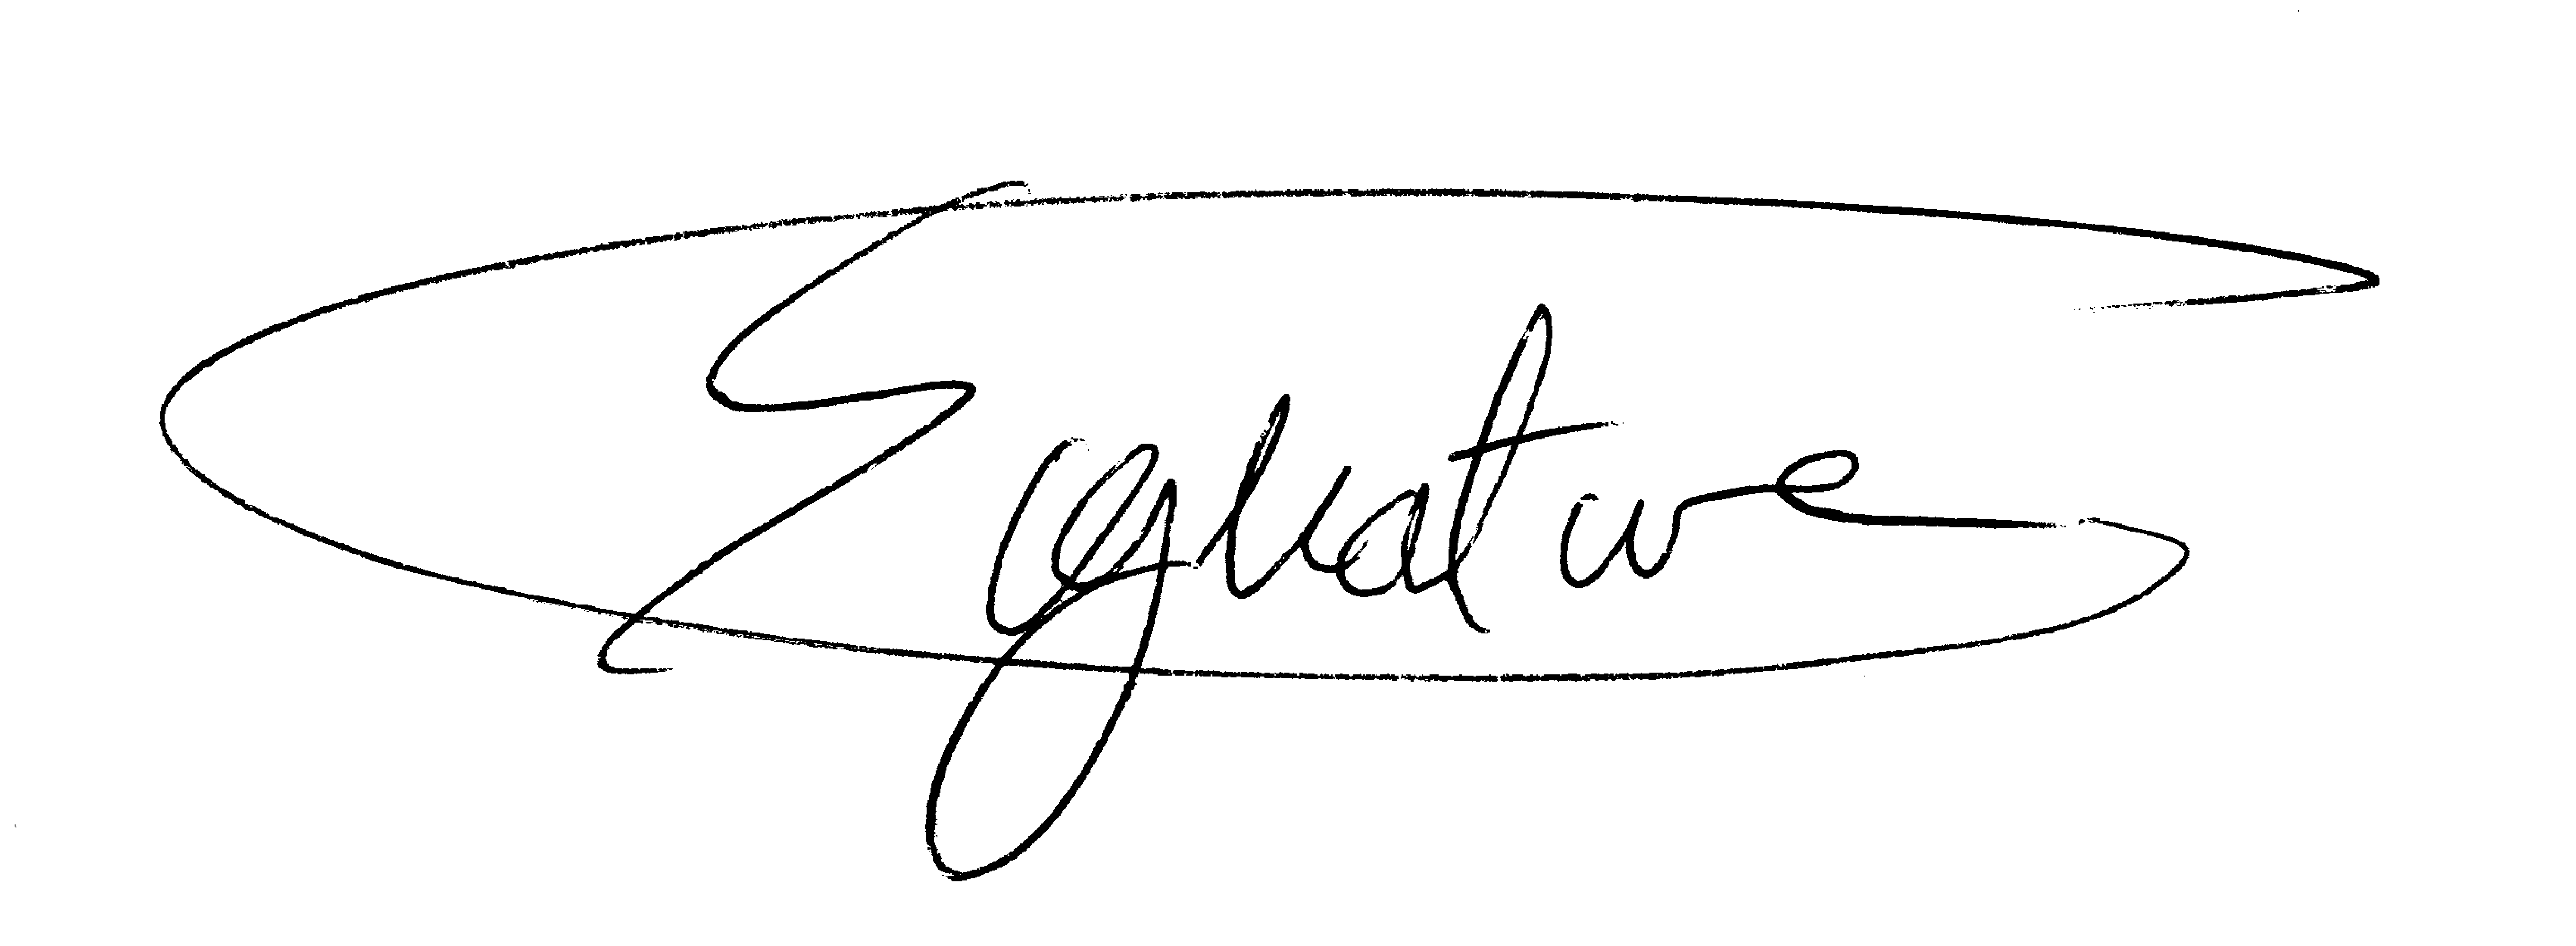
\includegraphics[scale=0.4]{Signature}\\[1cm]
\begin{flushright}
    \thesisauthor{}
\end{flushright}
}

	\pagestyle{scrheadings}	
		
	%*************************************************************
	% Mainmatter

	%*************************************************************
	\pagenumbering{arabic}
	%\setcounter{page}{90}
	% use \cleardoublepage here in case of problems with pdfbookmark

	\cleardoublepage\ctparttext{You can put some informational part preamble text here.}
	\part{Writing a Master thesis}

	\defaultfont

\BiChapter{����}{Introduction}
\label{Introduction}

\BiSection{���ⱳ��������}{The Background and Significance}
\label{Introduction:background}
\LaTeX~���ھ����Ű����ۡ��Թ�ʽ��ͼ���Ĵ�������ǿ���Լ���ƽ̨ͨ����ǿ�����ƣ�
ʹ�����ڿƼ��Ű��е�Ӧ��Խ��Խ�㷺��

\BiSection{����֪ʶ}{Mastering \LaTeX{}}
\label{sec:learningknowledge}
���ǵ�����ͬѧû�нӴ���~\LaTeX{}��Ϊ��������·���������֣�����ѧ��~\LaTeX{}�Ļ���ʹ�÷�����
�Ӷ��Ѹ����ʱ��Ͷ�뵽���ĵ�д�������У���רע�����ĵ����ݣ�������һ�ڽ���~\LaTeX �Ļ���֪ʶ��
�Ƽ�һЩ�ĵ����ϣ������õı༭���ɵ����ݡ�

\BiSubsection{ʲô��\LaTeX{}}{What is \LaTeX}
\label{sec:whatislatex}
        \TeX/\LaTeX ��һ�׹���ǿ���Ű������Ŀ���Դ�������Ѱ칫�Ű�������

        �Զ��ֲ���ϵͳ������~Microsoft Windows��\CJKglue Unix��~���磺Solaris��\CJKglue Linux �ȣ���\CJKglue
�Լ�~Mac OS X ��������Ӧ�����а汾��������Ҳ������ͬ���䷢չ���������ڻ���~linux ��
�˵��ڶ�~linux ����ϵͳ�ķ�չ���̡�

        ��~Windows ����õ���~\href{http://www.miktex.org}{MikTeX} ����������������װ��Linux ��������ò��ҳ������µ���
        TeXlive����ƽ̨��ijЩ�汾Ҳ������windows�£�����һ������ϵͳ~teTeX ���ֹͣ��ά����

        ��MikTeX�����ϣ�\href{http://www.ctex.org}{CTeX} ��~Aloft վ�������������������֧�֣�������~CTeX ������
װ����װ���ã���ȥ���û�������֮�࣬�Ƽ������û�����ʹ�á�

        ������������~��WYSIWYG��What You See Is What You Get�� ��~Microsoft Office
������ȣ������ص��ǣ�
   \begin{itemize}
      \item ���뼴����~��WYSTWYG��What You Think Is What You Get���������רע
�����ĵ�˼·��ͨ�����Ƿ��ӵĸ�ʽҪ�󣬸��ʺ��Ű�Ƽ����ģ�
      \item ���Ƹ�ʽ����,���������ݣ���ѧ��ʽ�����Ű淽��,���������
      \item ���ı��ļ�����������~MSWord �ĸ��ָ�ʽ�ױ䡢�ĵ��𻵡���ʽ�޷��༭�Ȳ��ȶ�����
      Ҳ�������ڰ汾���ƣ�
      \item �����~PDF �ļ��ǹ����ĵ���׼��������Ҫ��˶��ʿ��ҵ�����ύ��Ҳ��~PDF ��ʽ��
      \item �����ڿ�������һ�㶼�ṩ~\LaTeX ����ģ��,ʹ����Ͷ���Ű�����ף�
      \item Ŀǰ�����ⲻ�ٸ�УҲ������~\LaTeX{}ѧλ����д��ģ�壬ʹд��ѧλ���ĵ��Ű治����ʹ�࣬
      ����һ�����ܡ�������Ƚϳ���ļ�Ϊ��ģ�壻
      \item �����õ�Ƭ��~LaTeX ���~beamer���Ű湫ʽ����������һ�����㣬û��~PowerPoint
�����ַ�����ʽ��ͼƬλ�õ������ڶ��Ĭ��ģ�湩ѡ��һ��������Ϳ��л����ûõ�
Ƭ���������ɡ�רҵ��Ư����
      \item  �ڶ���ĵ���ͺ��֧�֣�����ĸо���``û�����������ģ�ֻ�����벻����''��
      \item  ��������ʵ��~TeXer ���ԣ�\TeX/\LaTeX �Ѿ���������һ���Ű�����������Ϊһ��������
      ��Ϊ���ĵ������䷢չ��������һ�����������Ĵ��档
    \end{itemize}

    �ܶ��˶���~\LaTeX{} �������ܣ�����Դ��϶����TeX����Ϊ~ 1 �����������ϼ�ҳ������У�ڵ�
    \url{ftp://202.118.224.241/software/Science/TeX&LaTeX/TeX\%20documents} ��Ҳ�м����õ�Ƭ���������˽��ܡ�
    �������߷����޸Ķ�Σ��������Ƽ���վ~\href{http://zzg34b.w3.c361.com/index.htm}{LaTeX�༭��} �ϵļ�ƪ���£�����ȫ���˽�����
   \begin{itemize}
     \item  \href{http://learn.tsinghua.edu.cn:8080/2001315450/tex_frame.html}{TeX���}������ʹ�õ�~\LaTeX ϵͳ�Ļ�����
     \item \href{http://zzg34b.w3.c361.com/homepage/TeXvirtue.htm}{TeX����ȱ��}: ���������������ǻ�����ʮȫʮ����
     \item \href{http://zzg34b.w3.c361.com/homepage/LaTeXbring.htm}{LaTeX�IJ���}�������ճ��Ӵ�����������
     \item \href{http://zzg34b.w3.c361.com/homepage/compareWord.htm}{LaTeXӦ�����}:���������������ڹ�����ʹ����Խ��Խ�ࡣ
     \item \href{http://zzg34b.w3.c361.com/homepage/compareWord.htm}{��Word��Ƚ�}:���������õ�����~word��~LaTeX�����߸����ŵ��ȱ�㣬��Ҫ�����ƫִ�Ĺ۵��У�����һƪ�ȽϿ͹۵����¡�
     \item \href{http://zzg34b.w3.c361.com/homepage/KnuthResume.htm}{Knuth ���ڼ���}:�ײ��ں�~ \TeX ������~ Donald Knuth (�ߵ���)�Ľ��ܣ����д���ɫ�ʣ�
     \item \href{http://zzg34b.w3.c361.com/homepage/LamportResume.htm}{Lamport ��ʿ����}�� \LaTeX ������~Lamport����������Ŭ��������~\LaTeX ʹ�ü򵥺ܶ࣬���ҿƼ��磻
   \end{itemize}

\BiSubsection{�Ƽ�������������}{LaTeX Software}
\label{sec:latexsoftware}

�������֣�Windows ��ֻ�Ƽ���ѵ�~CTeX ��װ����Ϊ˿������Ҫ�Լ����ã���װ��Ϳ���ʹ�á�
������У԰���û����Դ�~ \url{ftp://202.118.224.241/software/Science/TeX&LaTeX/CTex/} ����~
CTeX-2.4.5-8-Full.exe ��~ CTeX-Fonts-2.4.4.exe���Ȱ�װ��װϵͳ��Ȼ��װ���塣��У԰���û�
���Դ�~ \href{http://www.ctex.org}{CTeX�Ĺٷ���վ} �����������ļ���

\BiSubsection{�Ƽ�����������}{LaTeX Documents}

������ǵ�һ�νӴ�~ LaTeX����ô��װ~ CTeX ֮�󣬲�Ҫֱ�Ӵ򿪱༭����~WinEdt ���в�������Ϊ���������������˽⻹���٣��������ʴӡ����~ Windows
ϵͳ�Ŀ�ʼ~ $\rightarrow$ ����~ $\rightarrow$ ���� TeX ��װ~ $\rightarrow$ help $\rightarrow$
�����ĵ��˰ɣ����ǽ����˳���ǣ����ȴ�~ CTeX FAQ����ͷ����''��������''��һ�ڣ�Ȼ��
��ͬһĿ¼�´�~ LShort-cn �ļ�����ͷ��β�������һ�飬���ó��Լ�ס���е����
ֻҪ�˽�~ LaTeX ���ص㣬��ÿһ������һ��������ʶ�Ϳ��ԡ��Ժ��㻹���Ի�ͷ������������
Ȼ��� ~CTeX FAQ �����ϣ�����������У����Գ���ȥ��ϰ�Ű�һЩ�ĵ����鿴����Ч��������~ WinEdt ����
�����뿴����Ľ� \ref{sec:winedttricks}����

������⵽���������ĵ�~PDF: latex2e ��ͼָ�Ϻ�~mathematics (LaTeX ���� The LaTeX Companion ��~chapter8)��
�ֱ��ǽ���ͼ֪ʶ�͹�ʽ���뷽���ģ�������ϸ������Ҳ���һ�¡����ڹ�ʽ���룬����һ���ر�ֵ���Ƽ�����
\href{http://www.tug.org/tex-archive/info/math/voss/mathmode/}{mathmode 2.0}��У԰���û������Դ�
\href{ftp://202.118.224.241/software/Science/TeX&LaTeX/TeX documents/}{У��~FTP TeX ����Ŀ¼}���ء�

\BiSubsection{WinEdt�ı��뼰��������}{Winedt Tricks}
\label{sec:winedttricks}
~
��һ�ĵ�~ WinEdt\_LaTeX\_guide.doc �򵥽�����~ WinEdt �ļ��ĵ��ı��뷽�������Ե��
\url{http://bbs.hit.edu.cn/bbscon.php?bid=296&id=1887&ap=719} �õ���

������ϸ���ܱ��밴ť�ĺ��壬����һ�������ر���棬
��ע������Ľ���˳����~ WinEdt ��Ĭ������˳��
\begin{hitlist}
  \item TeX: ��������ʹ��~ TeX ����д���ĵ����ǵײ�ı���ϵͳ��
  \item LaTeX: ��������ʹ��~ LaTeX ����д���ĵ�����Ŀǰ����ʹ������~ LaTeX2e �ĵ�����ϵͳ������~ dvi �ļ���
  \item cct\& LaTeX: cct �ǹ��ڵ����ֲ��о�Ա������һ��ʹ��~ LaTeX �����������ĵ��Ľӿ�ϵͳ��
  ���Ȱ�~cct ���ĵ���~.ctx ת����~.tex ��ʽ��Ȼ����ñ�׼��~ LaTeX ����������dvi�ļ���
  \item PDFLaTeX: ����������~LaTeX������һ�ֱ���ϵͳ��ֱ������~pdf �ļ���֧�ָ����~ pdf �ļ���Ч������Ӧ��Խ��Խ�㷺���������Ļõ�Ƭ��
  \item BibTeX: ��������������ο����׵����ͨ��������һ�������ο�������Ŀ���б�~ bbl �ļ����Ű�ʹ�á�
  \item Make Index: ������������ĵ���������
  \item TeXify: ���Ǽ�����������ĺϼ������Զ�����~ LaTeX����pdflatex����MakeIndex ��~ BibTeX ��������Ҫ�Ĵ���������һ��
  ��������������б��ͽ������õ�~ dvi��pdf���ļ�������~ dvi��pdf���ļ������ɹ��̡�
  \item CTeXify: �����~ CTeX ��װ����������֧�ֵ�~TeXify ��������������ĵ�~ dvi(pdf) �ĵ���
\end{hitlist}

����ʹ���ĸ����밴ť��������ĵ����ͼ������������й�ϵ����Ϊ��ͬ�ı�����������ĵ��е�Ԫ��Ҫ��һ����
���磬��������õ���~eps ͼ�Σ�Ӧ����~latex�����룬����������~pdf ͼ�Σ�Ӧ����~pdflatex �����롣
�����������ǰ����ĵ���Ӧ��Ҳ�Ѿ������ˡ�

\BiSubsubsection{��ʾ�ĵ��ṹͼ}{File Structure Display}

WinEdt�е�~gather�����ռ��½ڱ��⣬�γ�~TOC �б�������������~word �е��ĵ��ṹͼ����
д���ĵ���ʱ��������ܷdz����ã����������ǵ�~Pluto ģ���У��Զ�����һЩ�½ڱ��⣬
��Щ�Զ������ȱʡ��~gather �Dz�ʶ��ġ�TeX@lilac �ṩ��һ�ַ�������~WinEdt.gdi�ж�����������
��Ч��ϣ����ʹ��������ܵ����ѿ����Լ������޸ģ�tools �ļ����������޸Ĺ���~WinEdt.gdi��
������Ҳ����ֱ��ʹ�ã��ŵ�~winedt Ŀ¼���滻ͬ���ļ����ɡ�

winEdt ��~ tree interfacezho ��Ҳ��~ TOC ��һ��������ͨ���޸� ~WinedtĿ¼�µ�~WinEdtEx.iniʵ�֡���~tools�ļ�����
��~WinEdtEx.ini �滻��ͬ���ļ��Ϳ��ԡ�

������Щ�Զ���������ڱ༭״̬�²�����ȱʡ����һ������������ܸ����ͺ��ˣ�TeX ͬ���ҵ����Լ�����ķ�����
��~winedt �˵�~ option/highlighting/switches �޸ģ�tools �ļ���~ Switches.dat ������
����õģ������������˵�λ��ʹ�öԻ���������~``Load from'' ��ť���ء�

\BiSubsection{����ͼ�ij�����ʽ}{Figure Generating}

��~latex �ĵ���д�����У����õ�ͼ�θ�ʽ��~ eps ��~ pdf ��

pdf �ļ����ɣ������úܶ��������ɣ�����~adobe acrobat ��pdffactory��pdf xchange �ȡ�
�����Ƽ�~ acrobat (ע�ⲻ��~ acrobat  reader)����Ϊ����װ������һ��~ pdf ��ӡ����
�κ�һ���ĵ�������ͨ�������ӡ������~pdf �ļ�������Ҫ�Ĺ����Ƕ�~ pdf �ļ��Ķ��༭��
pdf �ļ�������~acrobat ����вü�~ (documents,crop pages...)��ȡ������ҳ�档����֧��
ֱ������Ϊ~ eps �ļ��Ĺ��ܡ����ԣ�����~acrobat �������������е�ͼ�δ������ⶼ���Խ����
���������������ҵ������

������~latex ����ͼ�����Ƚ϶࣬���е���ͼ������~visio��~ coraldraw��~ photoshop��~ gnuplot ���ɵ�ͼ
������ͨ������ķ���ת����~eps ��~pdf �ļ������⣬���кܶ�ר��Ϊ~latex ��������ͼ������
��ͨ���������ʽ����ͼ�ģ�����~metapost��~pstricks��~asymptote��~pgf/tikz �ȣ�Ҳ�м򵥵�
������ͼ���������������~Dia��~winfig��~gclc �ȡ�  ��������������Щ����������ԱȽϼ򵥣�������ͼҲ����Ư�������Ƕ�û��΢����
~visio ��������ǿ�����Զ����������������~visio ����ͼ��

���ڲ�ͼ��������ڵ����İ��ͼָ���Ѿ�����ϸ�ˣ����ﲻ�ٽ��ܣ��뷭�ĸ��顣

\BiSubsection{�������д��ѧ��ʽ}{Math Inputting}

����һ��о���~LaTeX д��ʽ�Ƚ��鷳���Ӷ�����ȴ������ʵ������Դ�~mathtype����ҵ������
�������~ word �ﲻ�����Ļ�������������ѵ�~TeX ��ʽ����~TeXaids��ת���ķ�����
��~mathtype ��ʽ��������£�ѡ��˵��� ~``preference��translators...,translate to other language,
ѡ��~ TeX--LaTeX2.09 and later (��׼��LaTeX����)������~ TeX--AMS-LaTeX(��Ҫ~amsmaht ���֧��) ,ȷ�� ''
��Ȼ�����빫ʽ��ѡ�У����ƣ�ճ������ı༭����������빫ʽ�ĵط�����ῴ���������
��Ҫ�Ĺ�ʽ��~ LaTeX  ���룬�����Ϳ������������ˣ���ʱ������Ҫ����һ����ʹ�õ���ѧ�������ܴﵽ
���Ҫ��

�����������ѧ��ʽ��ʱ����������һ����ѧ���ţ����Ե������������ͷ���ͼ�꣬����ʾ
��ѧ���Ź�������Ȼ��������Ҫ����ѧ���ţ��Ͳ��뵽���ĵ��С�����һ��ר�ŵ�~symbol.pdf �ĵ���ctex
��װ��Ҳ�Ѿ��䱸���������еķ��ţ�����һЩϡ��Ź֣�������û�������ķ��ţ��������������ҵ���

ǰ���ᵽ��ctex ��װ��~help �ļ����Ѵ���~ch8.pdf ��~Mathmode.pdf �ļ��Թ�ʽ��д���ܵĺ���ϸ�����ָ����Ĺ�ʽ
������ͨ����ͬ����ѧ�����õ�������д��ʽʱ���ġ�

\BiSubsection{���ٲ���ͼ��}{Inserting Figures and Tables}

����ͼ���Ȼ����IJ��룬WinEdt �ṩ�˺������ķ�����ֻҪѡ�񹤾�����ͼƬ�ͱ���ť���Ϳ���
����һ��������ͼ���������Ҫ��ֻ�ǰ����е��ǺŻ����Լ��Ķ����Ϳ����ˡ�
WinEdt���ṩ��һ���꣬GUI ��ʽ���ͼ�IJ�����̣�ѡ����࣬Ҳ�����㡣
��ʱ�򣬸о�����Ƚϸ��ӣ���������~LaTeX д������Գ���һ�� ~xl2latex 2.0 ���~ excel
�������Ϊ~LaTeX ����ĺꡣ������~excel �����ɱ���Ȼ������һ�º꣬�������˱����~LaTeX ���롣
ģ���~edittools Ŀ¼���ṩ����һ�ļ���

\BiSubsection{���༼�ɼ����������ĵ�}{More Tricks and Others' Thoughts}

��������ż��ɣ����Բο��϶���TeX����õ׵�����~\href{http://bbs.hit.edu.cn/bbscon.php?board=TeX&id=2038&ftype=11}{���沿�����⵼��(��Ҫ����������)}��

	% \include{Chapter/MyOtherChapter}
	
	\cleardoublepage\ctparttext{Another informational part preamble text here.}
	\part{Using this Latex template}
	
	\renewcommand\thetable{\arabic{chapter}-\arabic{table}}
%\renewcommand\thefigure{\arabic{chapter}-\arabic{figure}} 
\chapter{結論與後續工作}
\label{cha:conclusions}


本論文蒐集了各類資訊安全工具軟體,目的是為了讓更多使用者了解資訊安全的重要性,以及如何更有效的運用網路資源。透過一系列的資訊安全基礎知識及專有名詞解釋,搭配軟體的安裝及實作步驟,讓初級使用者能更容易跨越資訊安全議題的門檻,對駭客攻防與妨駭相關知識有更深的了解。

對進階使用者而言,本手冊也針對開放源碼工具做介紹,大部分工具都有釋出其原始碼,並歡迎有能力的使用者開發出更完善的程式。另外,使用者也可以結合不同功能性的軟體,自行開發出一套符合其需求的軟體,例如利用作業系統辨識工具搭配弱點掃描工具,能夠更快的找出目標主機的系統漏洞,以發揮1+1大於2的功效。

\section{Future Work} 
%\paragraph{Future work} 
使用安全工具軟體開創一個美好和階的社會。


 
	
	% ************************************************************
	% Backmatter
	%*************************************************************
	\cleardoublepage%********************************************************************
% Bibliography
%*******************************************************
% work-around to have small caps also here in the headline
\manualmark
\markboth{\spacedlowsmallcaps{\bibname}}{\spacedlowsmallcaps{\bibname}}
%\phantomsection 
\refstepcounter{dummy} 
% to have the bib a bit from the rest in the toc
\addtocontents{toc}{\protect\vspace{\beforebibskip}}
\addcontentsline{toc}{chapter}{\tocEntry{\bibname}}
\label{app:bibliography} 
\printbibliography
	\appendix
	\cleardoublepage\part{Appendix}
	%********************************************************************
% Appendix
%*******************************************************
% If problems with the headers: get headings in appendix etc. right
\markboth{\spacedlowsmallcaps{Appendix}}{\spacedlowsmallcaps{Appendix}}
%************************************************
\chapter{Appendix example}

\begin{flushright}{\slshape    
    We have seen that computer programming is an art, \\ 
    because it applies accumulated knowledge to the world, \\ 
    because it requires skill and ingenuity, and especially \\
    because it produces objects of beauty.} \\ \medskip
    --- \citeauthor{knuth:1974}, \citetitle{knuth:1974},
\citeyear{knuth:1974} 
\end{flushright}

\section{The \texttt{listings} package to include source code}
Source code is usually not part of the text of a thesis, but if it is an original contribution it makes sense to le the code speak by itself instead of describing it. The package \verb!listings! provide the proper layout tools. Refer to its manual if you need to use it, an example is given in listing \ref{lst:probCounter}.

\lstinputlisting[
	firstline=1,
	lastline=47,
	float=tb,
	language=C++,
	tabsize=2,
	numbers=left,
	numberstyle=\tiny,
	stepnumber=2,
	numbersep=5pt,
	caption={Code snippet with the recursive function to evaluate the pdf of the sum $Z_N$ of $N$ random variables equal to $X$.}, 
	captionpos=t,
	label=lst:probCounter
	]{CodeFiles/probabilityCounter.cpp}

\end{document}
% ****************************************************************